\chapter{State of the Art} \label{chapter2}
    
    As Bill Gates, a famous American entrepreneur and co-founder of Microsoft Corporation, mentioned at a TED\footnote{https://www.ted.com/} conference in 2013, “\textit{We all need people who will give us feedback. That is how we improve.}” \cite{gates2013ted}. This simple phrase resonates with many of us. Regardless of the field in which a person activates and of their position, the lack of constructive advice decreases their ability to evolve from any perspective. 
    
    Despite expressing themselves freely, people tend to be hesitant to share their points of view \cite{hasan2012}. This behavior is mainly because individuals often gather truly negative remarks throughout their lives without being offered tips for improvement, thereby completely demotivating them. \cite{anna2011rowe}
    
    We examine the methods of offering and collecting feedback existing so far at \acrshort{acs}/\acrshort{upb} and develop feasible improvement solutions.

\section{Overview} \label{2:overview}

    According to Mary Clynes and Sara Raftery, "\textit{feedback represents an indispensable aspect of teaching and learning. People usually categorize terms used to describe feedback into two broad groups: constructive\slash corrective\slash negative and reinforcing\slash positive. In general, however, practitioners tend to use the terms negative or positive when describing feedback.}" \cite{mary2008sara}.
    
	Universities often offer opportunities to their students to share their impressions on different topics. These might range from verifying if the general endowment (more precisely location, hardware, and software support) is adequate for all activities carried out, how well prepared teachers are, and how captivating or challenging a class seems. Of course, besides remarks of the current situation of the educational environment, students are also encouraged to offer recommendations on how to improve the aspects considered as less pleasant or improper.
	
	However, although methods of submitting feedback to teachers are numerous \cite{musharraf2016sabina}, environments through which students can share their thoughts with future generations are limited and inconsistent. Concrete examples for the two previously mentioned categories concerning our university are further described in section \ref{2:existing_solutions}. Therefore, according to Eileen Ruberto \cite{ruberto2018chaos}, instead of having an organized platform or page containing the opinions of students, these are often ending up being shared in a chaotic style. As a result, she deduced that the likelihood that people might omit or lose specific comments or that the information handed over will not reach everyone who might be interested increases substantially.
    
\section{Case Study} \label{2:case_study}
    
    To observe the situation in the Romanian university education system regarding the feedback collection process closely, we interrogated several students from different cities and fields of study.
    
	A fourth-year student at the \textbf{\textit{Grigore T. Popa} University of Medicine and Pharmacy Iasi}\footnote{https://www.umfiasi.ro/en} that we interviewed mentioned that social platforms, i.e., Facebook or WhatsApp, are the main ways students share reviews about different topics. For instance, students have created private groups with all their fellows. These serve as a place where any student can address an inquiry, and someone else, who has already experienced that, might help him with an opinion or resolution. In addition, he confirmed that this method of sharing feedback is somewhat effective. However, it is time-consuming, given that information is not adequately structured and classified. In terms of providing feedback to teachers, similar to \acrshort{acs}/\acrshort{upb}, he uses the online course platform of his faculty to access a questionnaire at the end of each semester. However, in contrast to \acrshort{acs}/\acrshort{upb}, their survey extends over five weeks, occurring after the exam session. Moreover, the questions asked are primarily focused only on the capabilities of the teacher. Based on the results obtained from students, the university publishes an official list with the name of each teacher and its general score.
	
	A Master's degree student at the \textbf{Technical University of Cluj-Napoca}\footnote{https://www.utcluj.ro/en/} stated that distributing feedback in their institution is quite similar to the ideas previously listed. Hence, he is also using an online platform to select a specific class and its associated teacher, then being redirected to answer a set of anonymous questions. However, the authentication method represents an exciting aspect. More precisely, each generation of students needs to use a different generated code to login into the platform. Thus, at the end of the feedback period, students have absolutely no visibility on the statistics obtained.
	
	We also interviewed a fourth-year student at the \textbf{Faculty of Law}\footnote{https://drept.unibuc.ro/index-en.htm} within the \textbf{University of Bucharest}\footnote{https://unibuc.ro/?lang=en} (UB), howbeit the conclusion is the same: students cannot access the opinions and feedback submitted by their colleagues. As a result, social networks are located at the top in student collaboration and sharing impressions about different classes. 
	
\section{Existing solutions for our university} \label{2:existing_solutions}

    Universities have introduced various methods for students to express their reviews on various aspects of the educational process.

    Taking the Faculty of Automatic Control and Computers as an example, all possible channels of communication and argumentation of a point of view are:
    
    \begin{itemize}
                \setlength{\topsep}{0.5pt}
                \setlength{\itemsep}{0.5pt}
                \setlength{\parsep}{0.5pt}
                \item the \textbf{Moodle}\footnote{https://curs.upb.ro/?lang=en} course platform, which offers two possibilities: students can share their thoughts both on a forum dedicated to administrative information (throughout the whole semester) and at the end of a semester, through feedback questionnaires related to each class
                \item directly to teachers or assistants
                \item directly to the series guide
                \item constantly to the Computer Science \& Engineering Department, through the \textbf{LSAC}\footnote{https://lsacbucuresti.ro/} (Students League of Faculty of Automatic Control and Computers) association
                \item regular meetings organized by teachers, in which students express their thoughts about the academic year.
    \end{itemize}
    
    Thus, although there are many means through which students can express themselves to improve the teaching environment, there are no well-defined methods by which a current generation of students can provide a benchmark for future generations.
    
    Reviews passed between different generations of students are entirely disorganized: they share impressions via \textit{Google Docs}\footnote{https://docs.google.com/} or \textit{Google Sheets}\footnote{https://www.google.com/sheets/about/} files, distributed in groups formed on various social media platforms, like Facebook or WhatsApp. As a result, the risk of a student missing these reviews is enormous, considering situations such as failure to notice an essential post among dozens or hundreds of other messages, not belonging to the groups where feedback documents were published, or even the non-use of such social platforms.
    
	In the current context, in terms of feedback provided to teachers, especially using the Moodle platform, the main disadvantage comes from the fact that the data collection process does not provide transparency. Consequently, students do not know how it is handled, interpreted, and examined, the reason why they might feel their thoughts are not being taken into account.
	
	A study conducted by the \textbf{Faculty of Automatic Control and Computers} for two months, from March 2021 to May 2021, confirmed this theory. During this time, \textbf{1609} responses from both Bachelor’s and Master’s students, including all years of study, were collected. Hence, the data set obtained contains various opinions influenced by multiple factors, thus creating an unbiased coverage.
	
    This research revealed that about a third of the total students involved stated that they completed the feedback questionnaire at the end-of-semester, on average, at more than \textbf{75\%} of their classes, as illustrated in figure \ref{2:fig:number_classes_feedback_completed}: 
	
	\clearpage
	
	\begin{figure}[ht]
        \centering
             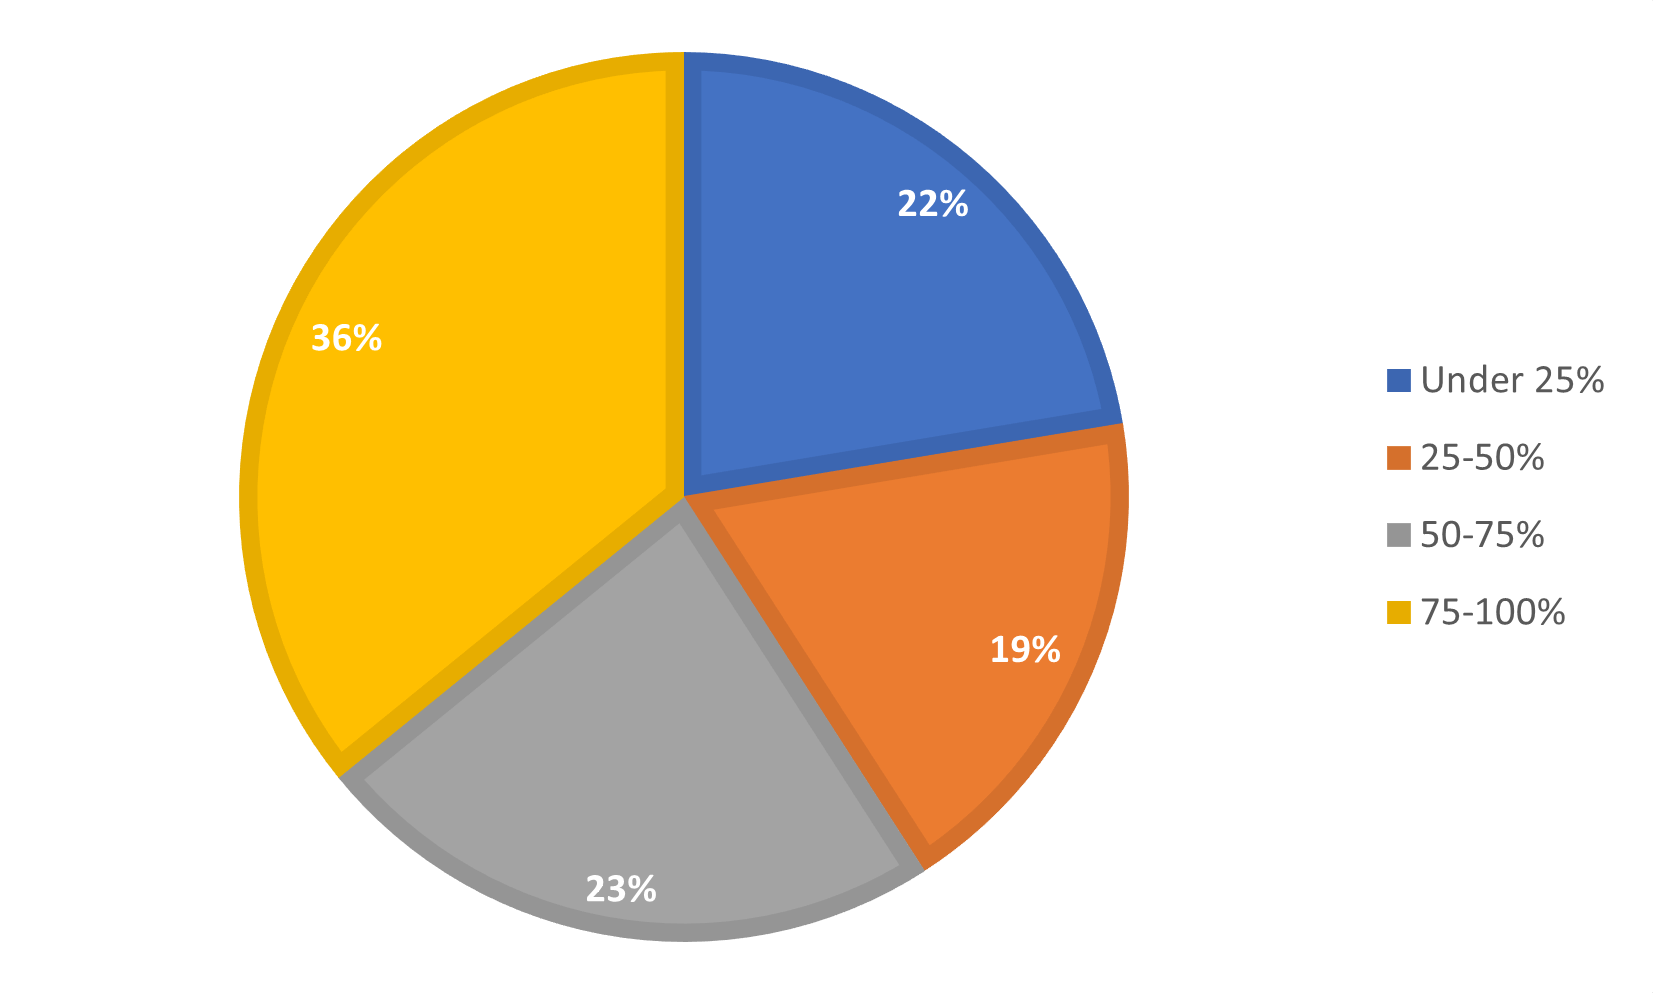
\includegraphics[height=0.3\textheight]{figures/charts/survey/number_classes_feedback_completed.png}
        \caption{Percentage of classes where students completed the feedback questionnaire at the end-of-semester}
        \label{2:fig:number_classes_feedback_completed}
    \end{figure}
	
	Asked why they choose not to complete such feedback questionnaires, \textbf{41,5\%} of the total number of participating students stated they do not believe these seem to impact. In addition, \textbf{33,8\%} mentioned that if a class is on the same page with their expectations and everything goes well, they prefer not to express their feedback anymore. On the contrary, among the least voted options are ideas that assume feedback is not anonymous or takes too long to complete. This outcome shows that students are confident their privacy is respected and data collected is not associated with a specific profile.
	
	Simultaneously, this study confirmed that the total time required to elaborate answers is not considered an impediment. However, another essential point of particular interest is that approximately \textbf{34.5\%} of students, being a rather worrying percentage, could identify other reasons (but these were not mentioned) for choosing not to get involved in such activities, as can be observed in figure \ref{2:fig:acs_survey_no_feedback}:
	
	\clearpage
	
	\begin{figure}[ht]
        \centering
             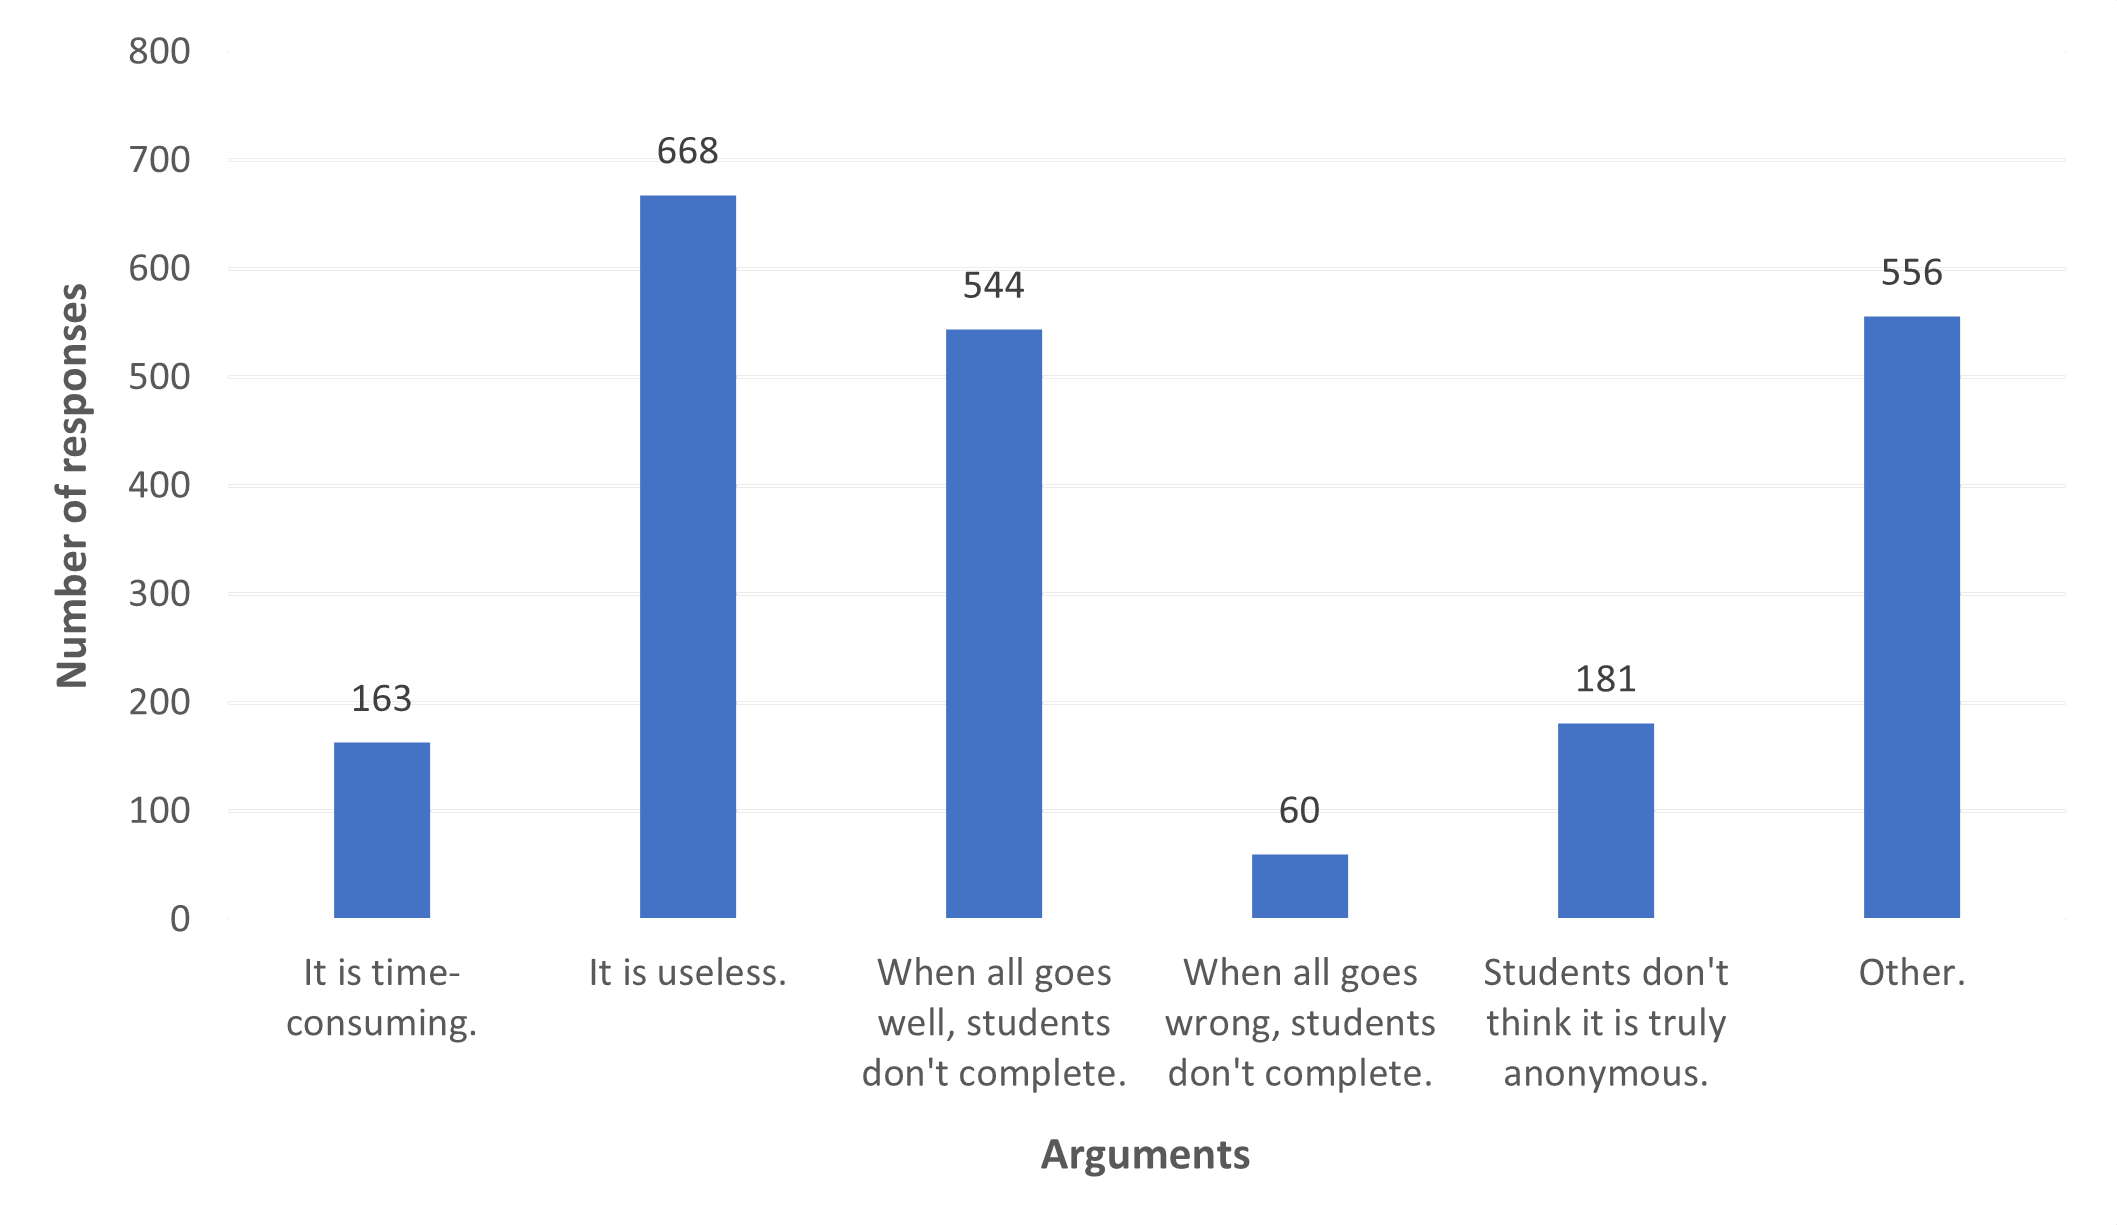
\includegraphics[height=0.4\textheight]{figures/charts/survey/acs_survey_no_feedback.png}
        \caption{Reasons for not completing the feedback form according to \textit{\acrshort{acs}/\acrshort{upb}}}
        \label{2:fig:acs_survey_no_feedback}
    \end{figure}
	
	Consequently, the purpose of this thesis is to outline as well as possible these ambiguities and analyze diversified solutions for their diminution.

\section{Feedback in pre-university environment} \label{2:preuni_feedback}

    In Romania, there is no clear strategy regarding the collection of feedback in the pre-university educational system. Equally, the perception of open communication between school students and teachers, combined with the exchange of mutual feedback, is almost non-existent. As a result, each teacher can maintain such activity only on his initiative since there is no regulation at a national level.
    
	Starting April 2021, under the guidance of the \textbf{National School Students Council}, the \textbf{Ministry of Education} is working on a methodology involving the evaluation of teachers and the atmosphere in classrooms at the end of each semester, via questionnaires that students can complete both electronically and in printed format. These are announced to be anonymous, and their processing is clearly expressed: data obtained will be used to identify the most effective teaching methods and how students perceive the benefits of education. Moreover, according to \textbf{Rareș Voicu}, President of the National School Students Council, the objective of this initiative will be to guide on how the didactic activities take place, thus signaling any dilemmas that should be treated \cite{cne2021feedback}. According to the Ministry of Education, after this law is approved, school students are given a chance to reflect regularly on how school aids them to advance and grow.
	
    In general, questions addressed to school students are highly similar to those intended for students at university, thereby improving the teaching-learning act. However, among the questions underlying this approach, different patterns can be identified: how clearly teachers explain the theory and the exercises, how high the workload is, whether the grading system is adequate or not, whether the overall difficulty is at an appropriate level, and how the teacher stimulates critical thinking.
    
	Therefore, since students are the beneficiaries of the educational system, they are the only ones capable of announcing what their needs, pleasures, and feelings are. The mission of each mentor is to feed the innate curiosity and intrinsic motivation of the students to strengthen their creative thinking and imagination.

\section{Other feedback sharing applications} \label{2:other_apps}

    People have developed various feedback applications over time, thereby craving to promote the free expression of thoughts and the act of offering suggestions.
    
	\textbf{Teleskop}\footnote{https://teleskop.ro/} is a cross-platform solution, delivered as a web platform or application for Android\footnote{https://www.android.com/} and iOS\footnote{https://www.apple.com/} operating system smartphones, allowing teachers to receive incognito feedback from students right at the end of each class. According to its founders \cite{teleskop10000}, over 10,000 answers were collected by the beginning of February 2021 from Romania and the Republic of Moldova. The main advantage of this application is that it is straightforward to use for both students and teachers:
	
	\begin{itemize}
            \setlength{\topsep}{0.5pt}
            \setlength{\itemsep}{0.5pt}
            \setlength{\parsep}{0.5pt}
            \item all needed is a device connected to the Internet
            \item completion time is as short as possible
            \item students do not need to authenticate
            \item a range of pre-configured forms can be selected directly
\end{itemize}
	
	Finally, all results are displayed in real-time straight into the account of a teacher, thereby being easy to apprehend.
	
	Furthermore, other tools that also aim to collect results, impressions, and thoughts are \textbf{Google Forms}\footnote{https://www.google.com/forms/about/} (one of the most used platforms at this moment), \textbf{Kahoot}\footnote{https://kahoot.com/} (which offers an interactive and pleasant environment through gamification features), \textbf{Socrative}\footnote{https://www.socrative.com/} (effective and easy to use application) or \textbf{Crowd Signal}\footnote{https://crowdsignal.com/} (a platform that specializes in creating customized questionnaires and allows the analysis of results).
	
	To get an overview of all the applications previously mentioned, we created a comparative table of features:
	
    \newcolumntype{P}[1]{>{\centering\arraybackslash}p{#1}}
	
	\begin{table}[th]\small\linespread{1}
        \centering
        \caption{List of features offered by other similar applications}
        \label{2:tab:comparative-table}
        \begin{tabular}{| l | c | P{1.5cm} | c | c | P{1.5cm} |}
        \hline
        \textbf{Feature} & \textbf{Teleskop} & \textbf{Google Forms} & \textbf{Kahoot} & \textbf{Socrative} & \textbf{Crowd Signal} \\
        \hline
        Anonymity & \Checkedbox & \Checkedbox & \Checkedbox & \Checkedbox & \Checkedbox
        \\
        \hline
        Cross-Platform & \Checkedbox & \HollowBox & \Checkedbox & \Checkedbox & \Checkedbox
        \\
        \hline
        Customizable questions & \HollowBox & \Checkedbox & \Checkedbox & \Checkedbox & \Checkedbox
        \\
        \hline
        Gamification & \HollowBox & \HollowBox & \Checkedbox & \Checkedbox &  \HollowBox 
        \\
        \hline
        Attractive \acrshort{ui} & \HollowBox & \HollowBox & \Checkedbox & \Checkedbox & \HollowBox
        \\
        \hline
        Real-time results & \Checkedbox & \Checkedbox & \Checkedbox & \Checkedbox & \Checkedbox
        \\
        \hline
        \end{tabular}
    \end{table}

\section{Coronavirus outbreak response} \label{2:covid_response}

    As a result of the pandemic situation generated by the \textit{SARS-CoV-2} virus, most universities in Romania decided to partially or wholly interrupt the physical activity of the classes, thus moving them to the online environment.
    
	Analyzing the environment within \acrshort{acs}/\acrshort{upb}, although this change was quite demanding at first, students have become accustomed to it. Feedback played a crucial role in determining how teachers conduct digital activities. After a year and a half of strictly supporting actions in a virtual climate, students stated through occasional meetings with the faculty management and coordinating professors that the overall level of tasks and involvement required has increased.
	
	Therefore, students were distressed that specific assessment methods had to be changed. Some classes were initially even forced to introduce more evaluations, thereby verifying knowledge gained. Fortunately, all these opinions were immediately collected and remedied as optimally as possible. In the same manner, teachers tried to offer increased flexibility to students. Thus, students were able to choose the variants most suitable for them. The final evaluation for some classes represents a clear example in this regard: students could choose whether they want to sustain the final examination in oral form, as an interview, or in writing. Oral exams were also a solution before the pandemic. However, these were rare, and students could not necessarily refuse them if these did not suit their pleasures.
	
	Even though face-to-face socialization was drastically reduced, our university provided students with sufficient communication channels so that their voices could be heard permanently. Therefore, the \textbf{Microsoft Teams} application is used for conducting online classes, and any issues encountered can be announced through a newly created ticketing system belonging to \textbf{UPB Support Center}\footnote{https://ticketing.upb.ro/open.php}.

\section{Motivation} \label{2:motivation}

    Throughout the last five years, feedback had a significant influence on \acrshort{acs}/\acrshort{upb} classes, both in terms of the curriculum taught and carrying out and evaluating activities. Naturally, the advice received from students was listened to and taken into consideration depending on different criteria, like veracity, or utility.
    
    Opinions received from students allowed teachers to continually refresh the content of their courses, to be up-to-date with the latest news and technologies on the market. On the one hand, this idea applies especially to technical engineering universities, given the fantastic progress in this area \cite{brian2009technology}, which might even occur from year to year. On the other hand, analyzing the situation of students that belong to other areas of expertise, for instance, medicine, history, or geography, it goes without saying that whether students fancy it or not, the curriculum cannot permanently be changed.
    
	\textbf{Systems Laboratory}\footnote{https://systems.cs.pub.ro/}, a team made up of professors, teaching assistants, and Ph.D. candidates from our university, emphasizes the importance of feedback. As a result, in addition to actively inspiring students to express their opinions, they always publish a report containing the data collected in a processed form, thus providing transparency for future generations. According to them, “\textit{this processing does not contain all the ideas, so as not to encourage a destructive attitude towards writing feedback. However, the team has received the entire raw feedback.}” \cite{wiki2020so}.
	
	Likewise, apart from the generic feedback questionnaire that students need to complete for each class on Moodle, teachers are also constantly elaborating other more particular surveys, which are focused strictly on the subject of their specific class. Hence, the desire to ameliorate the content of a discipline is quickly noticeable.
	
    As we have in mind all the information exposed throughout this chapter, we admit that feedback is an important note that underlies the evolution of each educational institution.